\subsection{$S$ 对偶}\label{sduality}

$\N=4$ 超 Yang-Mills 理论中一个特别简单的边界条件是规范场的 Neumann 边界条件，它以半 BPS 的方式延拓到整个超多重态。用膜的语言来说，这就是在规范理论 $\theta=0$ 时一族 D3 膜终止于单张 NS5 膜上的边界条件。

沿 $C$ 紧致化并约化到二维后，这个边界条件在 $\M_H$ 上给出一个膜 $\B_{\NS5}$，它对应于 $\M_H$ 上的平凡平坦线丛。换言之，膜 $\B_{\NS5}$ 的支撑是整个 $\M_H$，其 Chan-Paton 联络是平凡的。膜 $\B_{\NS5}$ 是 $(B,B,B)$ 型的，意味着它在每个复结构下都是 $B$ 膜。这反映了 $\M_H$ 上的平凡丛在每个复结构下都是全纯的。

在 $S$ 对偶（即电磁对偶）下，D3-NS5 边界条件被转换为 D3-D5 边界条件，$\theta$ 仍为零。另一方面，$S$ 对偶在维数约化后的理论中表现为 Hitchin 纤维的纤维上的 $T$ 对偶~\cite{BVJ,HM}。因此膜 $\B_{\NS5}$ 在 $S$ 对偶下必须映为支撑在 Hitchin 纤维化某个截面上的膜 ${\B}_{\uD5}$。此外，$(B,B,B)$ 型膜的 $S$ 对偶是 $(B,A,A)$ 型膜（这在文献~\cite{KW} 中已证明）。一个中间维数的膜要成为 $A$ 膜，其支撑必须是 Lagrangian 子流形，且其 Chan-Paton 丛必须是平坦的。因此 $\B_{\uD5}$ 所支撑的 Hitchin 纤维化截面从复结构 $I$ 的角度看必须是复 Lagrangian 的。另一方面，具体地说，单张 D5 膜情形的 D3-D5 边界条件由 $\t=1$ 处的 Nahm 极点描述~\cite{gw}。（这个 $\t$ 值对应于 $(B,A,A)$ 型未破缺超对称。）我们上面的分析确定了与 Nahm 极点相对应的 Hitchin 纤维化截面；它对应于 (\ref{equad}) 与 (\ref{varph}) 所描述的希格斯丛族。

% [Tutor Note: 物理图像] $S$ 对偶把 $(B,B,B)$ 膜变成 $(B,A,A)$ 膜，这一步是几何 Langlands 中“规范理论 $S$ 对偶 = Hitchin 纤维上的 $T$ 对偶（镜像对称）”的核心：$A$ 膜要求支撑为 Lagrangian 且 Chan-Paton 丛平坦，于是“$S$ 对偶像的支撑是 Hitchin 纤维化的截面且复 Lagrangian”就成了硬性约束，而不只是猜测。此处的截面正是 \cite{Hitchin} 的 Higgs 丛截面 $\T$，即 $\t=1$ 时 Nahm 极点对应的膜。

D3-NS5 边界条件可以通过引入 $\theta$、更一般地通过引入 NS5 膜上的 $U(1)$ 规范场来形变。这些形变在文献~\cite{gw} 中有描述，它们保持边界条件的半 BPS 性质，但会转动未破缺超对称。这一族中一个特定的形变（见文献~\cite{KW} 第 12 节）给出一个膜——典范余迷向膜 $\Bcc$——它在几何 Langlands 对应的规范理论进路中十分重要。$\Bcc$ 是支撑在整个 $\M_H$ 上的秩一膜，其 Chan-Paton 丛的曲率是 $\M_H$ 的各 Kähler 形式的线性组合。具体的组合依赖于一个类似于我们的 $\zeta$ 的参数。对几何 Langlands 方便的选择是取 Chan-Paton 丛的曲率为 $\omega_J$（复结构 $J$ 的 Kähler 形式）的倍数，此时 $\Bcc$ 是 $(A,B,A)$ 型膜。

% [Tutor Note: 约定差异] 膜的“型”按复结构 $(I,J,K)$ 的顺序记为三个字母，$A$/$B$ 分别指 $A$ 膜/$B$ 膜。$\Bcc$ 取 $(A,B,A)$ 意味着它对 $I$ 与 $K$ 是 $A$ 膜、对 $J$ 是 $B$ 膜；而 $\t=1$ 的 Nahm 极点给出的是 $(B,A,A)$。核对 $S$ 对偶给出的型时，务必先确认作者所用 $(I,J,K)$ 的排列次序，各文献（尤其 \cite{KW} 与本文）对三个字母的顺序约定并不总一致。

由 $\B_\NS5$ 形变得到 $\Bcc$ 的那个形变，其 $S$ 对偶是 $\B_\uD5$ 的一个形变，后者通过在 $\vec A$ 与 $\vec \phi$ 的场空间中转动 Nahm 极点得到。文献~\cite{gw} 分析了这一点，而第~\ref{motivation}~节曾简要描述了恰当的“转动”类型。正如我们已经看到的，转动后的 Nahm 极点边界条件导致一个支撑在 opers 簇上、即支撑在某个 $\zeta$ 对应的 $\V_\zeta$ 上的膜 $\Boper$。若按标准方式把 $\Bcc$ 定义为 $(A,B,A)$ 型膜，则其 $S$ 对偶必须具有相同的超对称。在那种情形下，$\Boper$ 支撑在通常的 opers 簇上，$\zeta=i$。（在本文中，$\zeta$ 取实值更为自然。）

% [Tutor Note: 易错点] 本段有两处易混：其一，$\Boper$ 的支撑是“opers 簇”$\V_\zeta$，而 opers 作为平坦丛的条件是“非分裂正合列”，它对复结构 $J$ 定义；当 $\zeta=i$ 时 $\V_{i}$ 才等于通常意义（关于 $J$）的 opers 簇。其二，$S$ 对偶保持超对称型，因此 $(A,B,A)$ 的 $\Bcc$ 的 $S$ 对偶仍必须是 $(A,B,A)$，这就把 $\zeta$ 钉死在 $i$；本文之所以偏好实数 $\zeta$，是因为后面的 Nahm 极点转动与第~\ref{simvar}~节的复对称破缺参数需要 $\zeta\in\R$。

$\Bcc$ 的 $S$ 对偶是支撑在 opers 簇上的膜 $\Boper$，这一事实在几何 Langlands 对应的数学处理中很重要。关于 opers 在几何 Langlands 对应中所起作用的解释，例如见文献~\cite{Frenkeltwo}。我们刚刚描述的事实给出了从规范理论理解 $\Bcc$ 与 $\Boper$ 之间 $S$ 对偶的途径。文献~\cite{NW} 论证了这两个膜之间的 $S$ 对偶对于理解 AGT 对应~\cite{AGT} 以及近期关于超对称规范理论与可积系统之关系的进展~\cite{NS} 都很重要。$\Bcc$ 与 $\Boper$ 之间 $S$ 对偶的作用在文献~\cite{NStwo} 中更为明确。

\subsection{单值性缺陷}\label{mondr}

希格斯丛的概念可以通过允许在孤立点 $p_i\in C$ 处出现奇点来推广。下文关心的是正则奇点的情形。为在 $C$ 中点 $p$ 附近引入正则奇点，我们在 $p$ 附近取 $C$ 上的局部复坐标 $z$，进而引入极坐标 $r,\theta$，$z=re^{i\theta}$。我们在极大环面 $T\subset G$ 的李代数 $\frak t$ 中选取元素 $\alpha,\beta,\gamma$，并寻找 Hitchin 方程在 $p$ 处具有如下形式奇点的解
\begin{align}\label{justo}A&=\alpha\,\d\theta+\dots \cr 
\phi&=\beta\frac{\d r}{r}-\gamma\,\d\theta+\dots \end{align}
其中省略号指比 $1/r$ 奇异性更弱的附加项。我们把这类余维二的奇点称为单值性缺陷。Hitchin 方程的一般理论很好地适用于这一情形~\cite{Simpson}，可以定义解构成的模空间 $\M_H(C;p,\alpha,\beta,\gamma)$，它是一个 hyper-Kähler 流形，其性质与没有单值性缺陷时相当类似。我们将要说的一切都以显然的方式推广到任意多个单值性缺陷的情形。

% [Tutor Note: 易错点] (\ref{justo}) 中 $\phi=\beta\,\d r/r-\gamma\,\d\theta$ 的两项量纲与角色不同：$\d r/r$ 项在 $r\to0$ 时发散（对数导数），它给出的是对称破缺方向（后面用于 blown-up $\sf A_1$ 奇点）；而 $\d\theta$ 项决定单值性。丢掉省略号（比 $1/r$ 更弱的项）后得到的单值性为 $U=\exp(-2\pi(\alpha-i\gamma))$，其中 $\alpha$ 来自 $A$ 的 $\d\theta$ 项、$\gamma$ 来自 $\phi$ 的 $\d\theta$ 项，符号与 $i$ 的位置需按 $A+i\phi$ 的约定核对。

一旦引入单值性缺陷，上面某些陈述对 $C$ 的亏格至少为 2 的限制就可以去掉。在存在足够多个单值性缺陷时，上述所有陈述对任意亏格的 $C$ 都成立（对 $G=SU(2)$，若 $C$ 亏格为 0 则所需数目为 3，若 $C$ 亏格为 1 则为 1）。

在 $\Sigma\times C$ 上的 $\N=4$ 超 Yang-Mills 理论中（$\Sigma$ 是另一个二维流形），可以考虑支撑在 $\Sigma\times p$ 上的单值性缺陷，其中 $p\in C$。Hitchin 方程的奇异解 (\ref{justo}) 自然地嵌入为四维方程 (\ref{bpseqns}) 的解。在 $C$ 相对于 $\Sigma$ 很小的极限下，$\Sigma\times C$ 上的 $\N=4$ 理论约化为 $\Sigma$ 上靶空间为 $\M_H(C;p,\alpha,\beta, \gamma)$ 的 sigma 模型。在这一描述中，还出现一个附加参数 $\eta$~\cite{GuW}，它是沿 $\Sigma\times p$ 未破缺的 $G$ 的阿贝尔子群的 theta 角。因此在量子层面，一个单值性缺陷实际上有四个参数 $\alpha,\beta,\gamma, \eta$。在 $S$ 对偶下，$G$ 规范理论中上述类型的单值性缺陷映为 $G^\vee$ 规范理论中类似的单值性缺陷。各参数在 $S$ 对偶下的变换为 $(\alpha,\eta)\to (\eta,-\alpha)$，而 $\beta$ 与 $\gamma$ 则作相应的标度变换（详见文献~\cite{GuW} 第 2.4 节）。

若丢掉 (\ref{justo}) 中由省略号表示的次领头项，我们发现复平坦联络 $\A=A+i\phi$ 的单值性为 $U=\exp(-2\pi(\alpha-i\gamma))$。只要 $U$ 是正则的——即 $G$ 中与 $U$ 对易的子群的维数等于 $G$ 的秩 $r$——次领头项就不改变单值性。若 $U$ 非正则，则有一个重要的微妙之处，文献~\cite{GuW} 第 3.3 节对此有详细解释。为简洁起见，这里只考虑 $G=SU(2)$ 的情形，此时 $U$ 的非正则取值只有 $\pm 1$。若 $U=\pm 1$，则形如 (\ref{justo}) 的联络的单值性 $V$ 未必与 $U$ 共轭；相反，它一般落在包含元素
\begin{equation}\label{zonk}U'=\pm \begin{pmatrix}1 & 1 \cr 0 & 1 \end{pmatrix}.\end{equation}
的“幂幺”共轭类中。该共轭类的一般元素 $V$ 是 $\pm 1$ 加上一个任意幂零矩阵：
\begin{equation}\label{onk}V=\pm 1 + \begin{pmatrix} x & y \cr z & -x \end{pmatrix},~~x^2+yz=0.
\end{equation}
方程 $x^2+yz=0$ 描述一个 $\sf A_1$ 奇点 $\C^2/\Z_2$。奇点位于 $x=y=z=0$ 处，那里单值性 $V$ 恰为 $\pm 1$；换言之，这正是 (\ref{justo}) 中的次领头项不修正单值性的情形。在把 $\alpha$ 与 $\gamma$ 取为使 $U=\pm 1$ 的特殊值时，我们将假定 $\beta$ 仍为一般值。此时即使 $U=\pm 1$，解也内建了一个“对称破缺方向”，由联络中正比于 $\beta$ 的奇异项给出。其效应是吹开 $\sf A_1$ 奇点，把 $\C^2/\Z_2$ 换成 $T^*\CP^1$。这一重要事实在文献~\cite{Simpson} 中确立。

这个 $T^*\CP^1$ 的确切含义是：若 $U=\pm 1$ 且 $\beta=0$，则 $\M_H(C;\alpha,\beta,\gamma)$ 有一个 $\sf A_1 $ 奇点轨迹，它参数化那些绕 $p$ 的单值性恰为 $\pm 1$ 的希格斯丛。但若 $\beta\not=0$ 而 $U$ 仍等于 $\pm 1$，则这条奇异轨迹被吹开，奇点被一族 $\CP^1$ 取代。

模空间 $\M_H(C;p,\alpha,\beta,\gamma)$ 在把 $\alpha$ 平移一个余特征标（cocharacter）下不变——对 $G=SU(2)$，这意味着它在 $\alpha\to \alpha+\mathrm{diag}(i,-i)$ 下不变，而这个平移可以由一个在 $p$ 处有奇点的规范变换诱导。然而，我们感兴趣的是不具有这种 $\alpha$ 平移不变性的膜构造，因此就本文目的而言，最好不把 $\alpha$ 看作周期变量。

% [Tutor Note: 物理图像] 为什么 $\alpha$ 的平移可以由“在 $p$ 处有奇点的规范变换”实现：$\alpha$ 是 $A$ 的 $\d\theta$ 系数，绕 $p$ 一圈的规范变换 $g=e^{i\theta\,\mathrm{diag}(1,-1)}$ 把 $\alpha$ 平移一个余特征标，同时在 $p$ 处留下奇点。膜构造之所以不保持这一平移，是因为在膜的语言中 $\alpha$ 对应 NS5 膜的位置/相位，平移它需要移动膜，而非仅仅作规范变换。

\begin{figure}
 \begin{center}
     % >>> 原文图 26（原稿第 104 页）
  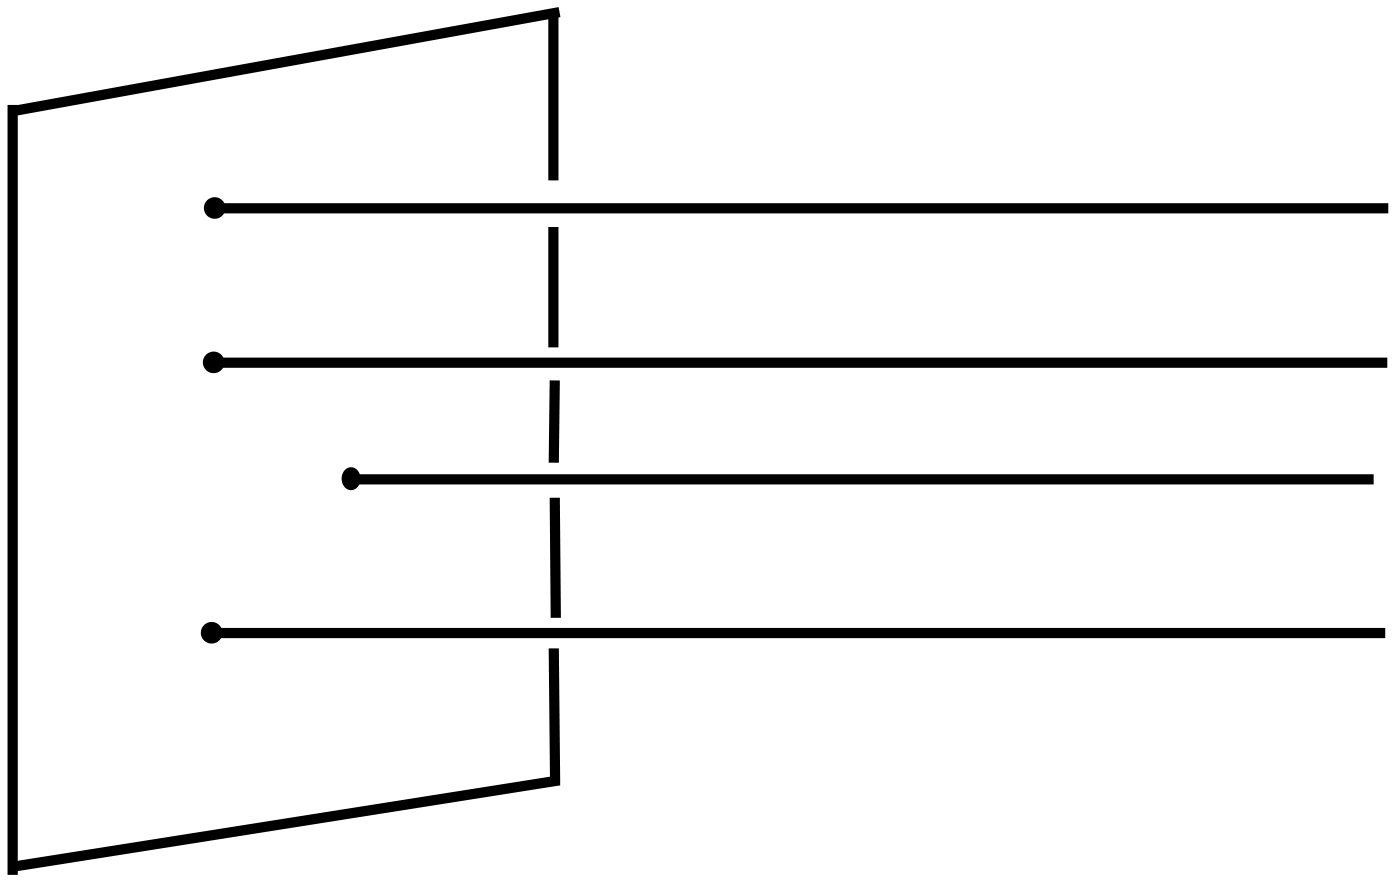
\includegraphics[width=3.5in]{figs/Fig26.png}
 \end{center}
\caption{\small  $C\times \R_+$ 中的单值性缺陷，支撑在 $p_i\times \R_+$ 上，其中 $p_i$ 是 $C$ 中的点。$C$ 用矩形表示。我们假定 $y=0$ 处有 Nahm 极点边界条件。（原稿第 104 页）}
 \label{defects}
\end{figure}
我们要考虑的第一个膜是 oper 膜。它照例由 Nahm 极点边界条件定义。为此取 $\Sigma$ 为 $\R\times \R_+$，其中 $\R_+$ 是通常的半直线 $y\geq 0$，并在 $y=0$ 处施加 Nahm 极点边界条件。略去 $\R$ 即时间方向，$C\times \R_+$ 上的图像如图~\ref{defects} 所示：有支撑在 $p_i\times \R_+$ 上的单值性缺陷，各自带有参数 $(\alpha_i,\beta_i,\gamma_i,\eta_i)$，以及 $y=0$ 处的 Nahm 极点边界条件。当然，我们需要解释：当单值性缺陷终止于带 Nahm 极点的边界上时，我们想要的是何种奇点。一如往常，这类问题可以通过寻找具有所需奇点的模型解来回答。就目前情形而言，文献~\cite{fiveknots} 第 3.6 节已经做了这件事，文献~\cite{Mikhaylov} 则给出了更一般的处理。

设 $\alpha-i\gamma=\lambda\,\mathrm{diag}(i,-i)$，$\lambda$ 为复参数，并考虑在（比如）$z=0$ 处具有这类奇点的希格斯丛 $E$。若 $E$（在复结构 $I_\zeta$ 中看）同时也是一个 oper，则它可由经典应力张量
\begin{equation}\label{lork}t=-\frac{\lambda(\lambda+1)}{z^2}+\dots, \end{equation}
描述，其中我们略去了奇异性更弱的项。这个公式与 (\ref{roog}) 相似，只是把 $j_a=k_a/2$ 换成了 $\lambda$。$E$ 的平坦截面对应于微分方程
\begin{equation}\label{stork}\left(\frac{\partial^2}{\partial z^2}+t\right)\psi=0.\end{equation}
的全纯解。对一般的 $\lambda$，可以找到两个线性无关的解，$\psi_1=z^{-\lambda} \left(1+\sum_{i=1}^\infty c_iz^i\right)$，$\psi_2=z^{\lambda+1}\left(1+\sum_{i=1}^\infty \tilde c_i z^i\right)$。这意味着，正如预期，单值性为
\begin{equation}\label{dusc}U=\mathrm{diag}(\exp(-2\pi i\lambda),\exp(2\pi i\lambda)).\end{equation}

% [Tutor Note: 物理图像] (\ref{lork}) 中的组合 $-\lambda(\lambda+1)/z^2$ 正是二维共形场论中“权重为 $j=-\lambda-1$ 与 $j=\lambda$ 的退化场”所对应的应力张量零点结构（比较 (\ref{roog}) 中 $j_a=k_a/2$ 的情形），它保证 (\ref{stork}) 有 $z^{-\lambda}$ 与 $z^{\lambda+1}$ 两个解，指数之和为 1。$\lambda\to k/2$ 时两指数之差 $2\lambda+1\to k+1$ 成为整数，于是出现对数解——这正是下一段要处理的情形。

若改为取 $\lambda=k/2$，$k\in \Z$，会怎样？此时总存在解 $\psi_2=z^{k/2+1}(1+\sum_{i=1}^\infty \tilde c_iz^i)$，但若我们寻找形如 $\psi_1=z^{-k/2}(1+ c_1z+\dots)$ 的解，就会发现：一般地，当把该展开推进到 $z^{k/2+1}$ 阶时，我们需要量级为 $ z^{k/2+1}\log z+\dots$ 的对数项。对数项恰好是 $(\log z)\psi_2$ 的某个倍数。相应地，绕 $z=0$ 的单值性一般地取幂幺形式
\begin{equation}\label{omogg}
\begin{pmatrix} \psi_1\cr \psi_2\end{pmatrix}\to (-1)^k\begin{pmatrix} 1 &  s\cr
    0 & 1\end{pmatrix}\begin{pmatrix}\psi_1 \cr \psi_2\end{pmatrix}\end{equation}
    其中 $s$ 为某个复常数。

因此，若要使绕 $z=0$ 的单值性为平凡，我们需要对 (\ref{lork}) 应力张量的次领头系数施加一个条件，以使 $s=0$。这意味着：绕 $z=0$ 的单值性平凡是一个中间维数的条件。确实，若无此条件，$G=SU(2)$ 的单值性缺陷使 $\M_H$ 的复维数增加 2，而平凡单值性条件固定这 2 个参数中的 1 个。

% [Tutor Note: 省略论证] 作者说“$s=0$ 是对次领头系数的一个条件”而未写出显式公式：具体地，$s$ 是应力张量中 $1/z$ 阶项（即 $t=-k(k+2)/(4z^2)+t_{-1}/z+\dots$ 中的 $t_{-1}$）的线性函数；把 (\ref{stork}) 的 Frobenius 级数推进到对数阶即可解出 $s\propto t_{-1}$。因此“平凡单值性”在参数空间中确实是一个余维 1 的条件，这正是“中间维数”的定量含义。

这一点很重要，我们稍作展开。一般地，绕缺陷的单值性是 $SL(2,\C)$（复维数 3）中满足一个约束（指定其共轭类）的元素，从而剩下 2 个复参数。例如当 $\alpha=\gamma=0$ 时，该共轭类是二维的，正如 (\ref{onk}) 所显式展示的那样。平凡单值性条件（仅当 $U=\exp(-2\pi(\alpha-i\gamma))$ 等于 $\pm 1$ 时才有定义，对其他取值没有类似物）固定与缺陷相联系的 2 个参数中的 1 个，于是剩下 1 个参数。可以把这 1 个参数看作式 (\ref{justo}) 中 $\beta \,\d r/r$ 项所对应的对称破缺方向。对称破缺方向的选取确定了一副本 $\CP^1$ 中的一个点；这个 $\CP^1$ 是 $E$ 在单值性缺陷所在点 $p\in C$ 处的纤维的射影化。关于这个 $\CP^1$ 之来历的更详细解释如下。首先，由于方程 $x^2+yz=0$，式 (\ref{onk}) 所描述的幂幺共轭类作为复流形显式同构于 $\C^2/\Z_2$，在 $x=y=z=0$ 处有 $\sf A_1$ 奇点。该奇点正是 (\ref{onk}) 中群元 $V$ 等于 $\pm 1$ 的那个点。在把 $\M_H$ 构造为 hyper-Kähler 流形的框架中，$\beta$ 参数是吹开 $\sf A_1$ 奇点的 Kähler 参数，它把共轭类 $\C^2/\Z_2$ 换成其消解，即 Eguchi-Hansen 流形 $T^*\CP^1$。在吹开中，原点处的奇点被一份 $\CP^1$ 取代。关于 $\beta$ 作为吹开参数的解释见文献~\cite{Simpson}，关于其中若干事情的从容解说见文献~\cite{GuW}。

% [Tutor Note: 原文用词] 原文写作 “Eguchi-Hansen manifold”，通行拼法为 Eguchi-Hanson（埃古奇–汉森空间）。此处按原文保留，未作改动；它指 $T^*\CP^1$ 作为 $\C^2/\Z_2$ 的极小消解所带的 hyper-Kähler 度规。

我们实际上已经遇到过如下事实：在这一情形中，单值性消失是一个中间维数的条件。我们专门考虑 $C=\CP^1$ 的情形（我们也可以类似地处理 $C=\C$ 且在无穷远处有非正则奇点的情形）。由第~\ref{opbethe}~节我们知道，对给定的一组奇点 $z_a$ 与磁荷 $k_a$，$a=1,\dots,d$，只有有限多个具有无单值性奇点的 oper。平坦 $G_\C$ 丛成为 oper 这一条件是中间维数的条件。要归约为有限多个具有无单值性奇点的 oper，单值性消失的条件也必须同样是中间维数的。（这一断言暗中假定两个条件以横截的方式相交，事实确实如此。）

事实上，若放弃 oper 条件，我们可以显式描述 $C$ 上 Hitchin 方程解构成的模空间，其中单值性缺陷由 $\lambda_a=k_a/2$ 刻画，且复联络 $\A$ 绕这些点的单值性平凡。由于 $C$ 单连通，$C$ 上绕各点 $p_a$ 无单值性的平坦丛作为平坦丛是完全平凡的。唯一可能的模来自与参数 $\beta_a$（我们假定全部非零）相联系的对称破缺：它在每个奇点 $p_a$ 处生成一份 $\CP^1$。要得到模空间，必须把这些 $\CP^1$ 的乘积除以平凡平坦丛 $E$ 的自同构群；后者是一份 $SL(2,\C)$。于是最终，Hitchin 方程在各奇点处单值性平凡的平坦丛所对应的解构成的轨迹 $\mathcal U$ 同构于 $(\CP^1)^d/SL(2,\C)$。这是 $\M_H$ 在复结构 $J$ 下的一个复子流形（它由对单值性的条件定义，而单值性在该复结构下是全纯的）。其维数为 $d-3$，恰为 $\M_H$ 维数的一半。事实上，从复结构 $J$ 的角度看 $\mathcal U$ 是复 Lagrangian 的；这大致是因为每份 $\CP^1 $ 在 $T^*\CP^1$ 中都是复 Lagrangian 的。因此，支撑在 $\mathcal U$ 上、带平凡 Chan-Paton 丛的膜 $\Btriv$ 是 $(A,B,A)$ 型的半 BPS 膜。

% [Tutor Note: 易错点] 维数核对：$(\CP^1)^d$ 复维数 $d$，除以 $SL(2,\C)$（复维数 3）得 $d-3$。而 $\M_H$ 对 $G=SU(2)$ 的复维数为 $6(g-1)+2d=2d-6$（$g=0$，$d$ 个正则奇点），其一半正是 $d-3$。注意此处 $g=0$ 时先要 $d\ge3$ 才能整除得到正维数，这与前文“亏格 0 需 3 个单值性缺陷”的说法一致。

这给了我们思考平凡单值性 opers 的新方式。它们是两个 $(A,B,A)$ 型 Lagrangian 子流形的交点——一个流形是 opers 簇，另一个参数化具有平凡单值性的丛。因此，平凡单值性 opers 给出拉伸在膜 $\Boper$ 与膜 $\Btriv$ 之间的超对称开弦空间的一组基。我们称这个空间为 $(\Boper,\Btriv)$ 弦空间。技术上，这里我们要的是 $J$ 型 $B$ 模型中的 $(\Boper,\Btriv)$ 弦空间。

我们可以利用 $S$ 对偶来研究这个超对称弦态空间，$S$ 对偶把 $J$ 型 $B$ 模型转换为 $\omega_K$ 型 $A$ 模型。正如第~\ref{sduality}~节所知，$S$ 对偶把膜 $\Boper$ 转换为典范余迷向膜 $\Bcc$。结果表明（我们将很快描述），$\Btriv$ 在 $S$ 对偶下映为自身（单值性缺陷参数 $(\alpha_a,\beta_a,\gamma_a,\eta_a)$ 按通常方式变换）。因此 $(\Boper,\Btriv)$ 弦空间的 $S$ 对偶就是 $(\Bcc,\Btriv)$ 弦空间，只不过现在是在 $\omega_K$ 型 $A$ 模型中看。这个问题的关键之处在于：虽然 $\Btriv$ 的支撑对 $\omega_K$ 是 Lagrangian 的，但它对 $\omega_J$ 实际上是辛的——确实，$\Btriv$ 的支撑是复结构 $J$ 下的复子流形，因而以 $\omega_J$ 为其 Kähler 形式。既然如此，描述 $(\Bcc,\Btriv)$ 弦空间的问题就由文献~\cite{GuWtwo} 中关于量子化与膜的分析所支配。$(\Bcc,\Btriv)$ 弦空间通过量子化 $\Btriv$ 的支撑 $\mathcal U$ 得到；这里 $\mathcal U$ 被视为带辛结构 $\omega_J$ 的辛流形。



 \begin{figure}
 \begin{center}
     % >>> 原文图 27（原稿第 106 页）
  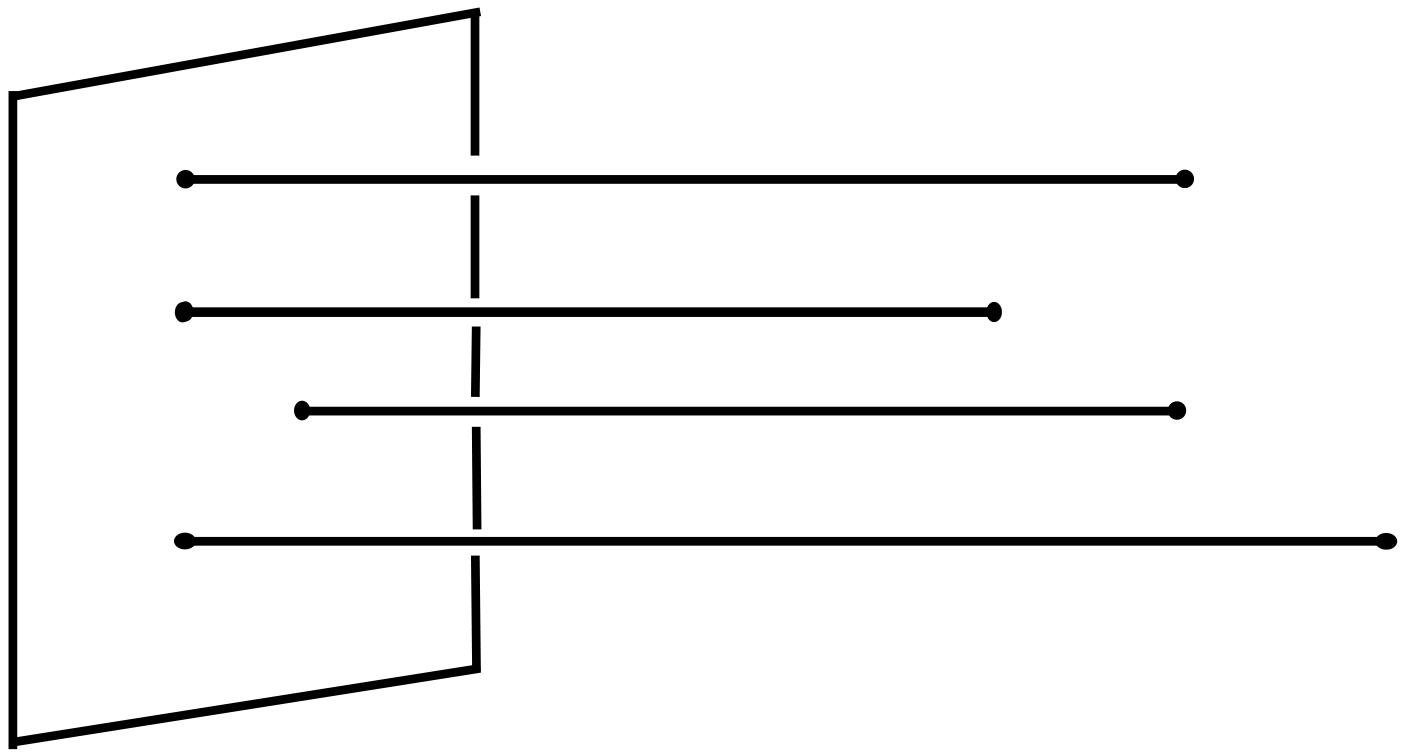
\includegraphics[width=3.5in]{figs/Fig27.png}
 \end{center}
\caption{\small  本图与图~\ref{defects} 的唯一区别在于：每条单值性缺陷线都终止于一个奇异磁单极子，即右侧的黑点。由于缺陷线本身是自对偶的（在参数作适当变换之后），由缺陷线终止所定义的膜也是自对偶的。（原稿第 106 页）}
 \label{ends}
\end{figure}

\subsection{一个自对偶膜}\label{simplex}
关于 $\Btriv$ 为何自对偶，有一个简单的规范理论解释。暂时不管超对称，我们可以把单值性缺陷线看作与一个可能未被正确量子化的磁单极子相联系的 Dirac 弦。因此，单值性缺陷线可以终止于一个奇异磁单极子（图~\ref{ends}）。由于单值性缺陷在 $S$ 对偶下映为自身（参数作某种变换），单值性缺陷终止于奇异磁单极子的图像在 $S$ 对偶下也类似地映为自身。

超对称对这类图像得以存在的参数取值施加了一些约束。在 $J$ 型 $B$ 模型的框架中，若缺陷线要终止，则绕给定缺陷线的单值性必须平凡。这意味着，在这个 $B$ 模型中，图~\ref{ends} 的图像只有在 $\alpha=\gamma=0$ 时才存在（这里我们把 $\alpha$ 与 $\eta$ 视为周期变量）。当然，无论如何那都是 $\Btriv$ 得以定义的情形。对偶地，在 $\omega_K$ 型 $A$ 模型中，像图~\ref{ends} 那样的图像只有在 $\gamma=\eta=0$ 时才存在。（例如，$\eta$ 必须为零，因为若单值性缺陷的支撑终止于沿该缺陷的 $U(1)$ 丛未被平凡化的地方，则世界面 theta 角 $\eta$ 就不能保持 $A$ 模型的拓扑超对称。）



在本文的框架中，具有平凡单值性的 opers 最直接地来自 $y=0$ 处的奇异磁单极子。不过，在不改变任何本质内容的前提下，我们可以把奇异磁单极子移离边界，只要用单值性缺陷把它们与边界相连，如图~\ref{ends} 那样。这样做的好处是：它使“平凡单值性 opers 是两个膜的交点”这一点变得显然，也使其中一个膜的自对偶性变得清楚。

在缺陷线终止于奇异磁单极子的一般情形中，该磁单极子可能被错误地量子化。然而对 $\lambda=k/2$，它等价于 $\gamma=0$、$\alpha=(k/2)\mathrm{diag}(i,-i)$，此时弦末端的磁单极子服从 Dirac 量子化，但该弦是可观测的，因为我们假定 $\beta\not=0$。
